\chapter{Introduction}

\section{Understanding Participation in Science Education}
There has been an increasing drive to address issues surrounding equity and access in science education. Much research has shown that educational interests in science and technology have declined over time \citep{OECD2006}. In addition, there tends to be uneven levels of interests and retention in science and technology across various demographic characteristics, including ethnicity, gender \citep{cheryan2017some,su2015all}, and Socio-Economic Status (SES). Across the world, there is increasing demand to address these inequities. In New Zealand, the need to address inequities are particularly salient for government. As outlined in the Child Youth and Wellbeing Strategy \citep{wellbeing2019}, it is important that young people are not only learning and developing, but they are doing so in a way that ensures that they are happy and healthy. Te Tiriti o Waitangi (The Treaty of Waitangi) also sets out a requirement for intergenerational inequities to be addressed regarding M\={a}ori \citep{treatywaitangi}, the indigenous population of New Zealand who still suffer from the impact of colonisation. When applied to the field of science education, researchers and policy makers are thus charged with understanding and addressing disparities related to science participation, achievement, and interests. 

Research into inequities in STEM often focuses on one aspect of an individuals identity, with the cost of sacrificing an intersectional perspective that can provide more understanding of each individual's unique life circumstances. Forsaking an intersectional approach can lead to the life experiences of certain groups going unreported and unheard. There is an increasing wealth of literature detailing gender disparities in STEM interests and outcomes \citep{Sue2009,wang2017gender}, but there are relatively fewer studies that explore intersections with ethnicity \citep{fouad2017scct,grossman2014perceived}, and even fewer still that investigate the intersections between gender, ethnicity and social class \citep{archer2013aspires}. Many researchers are now advocating for intersectional approaches to understand student experiences in STEM and at university \citep{jury2017experience}. It is also important to consider that, while it can be relatively simple to operationalise gender and ethnicity (i.e., through self-identification), social class is a more difficult construct to define and operationalise. Socio-economic status is the most commonly used indicator of social class, but as argued by \cite{rutkowski2013measuring}, a `one size fits all' approach to SES can be criticized for neglecting cross-country and cross-cultural differences. This argument can be extended further by exploring how social class relates to a students specific field of study or career intention. While having parents with highly paid jobs has been shown to be beneficial for students across different contexts, research has also shown that parents employment is linked to domain-specific preferences in education. Children who have parents who work as scientists are more likely to grow up study science themselves \cite{moakler2014college}, with this being especially true in physics \citep{upshot}. Recent research in science education has applied Pierre Bourdieu's sociological theory of taste to operationalise social class in terms of cultural and social capital \citep{Archer_2015}. These concepts not only provide a method of conceptualising social class that realises the social, cultural, and historical contexts in which individuals are placed, but it also provides an underlying theoretical framework that details how social class intersects with other aspects of identity (i.e., across axes of ethnicity and gender). 

As noted by theorists, capital by its very nature is not distributed evenly across society. Students from less affluent backgrounds tend to have poorer educational outcomes \cite{May_2016}, and are less likely to realise tertiary education goals \cite{reynolds2011change}. Students who do not have parents or family members who attended university face additional challenges in adapting to life at university. 

In New Zealand access to capital is disproportionately distributed across ethnic groups. M\={a}ori and Pasifika students are over represented in low SES areas (an ongoing consequence of New Zealand's colonial history), subjected to everyday racism and discrimination \citep{mayeda2014you}, and are the subject of lower academic expectations from teachers \citep{turner2015teacher}. Given these findings, it is not surprising that research shows that M\={a}ori and Pasifika students are less likely to be retained in university study, with especially true with regards to scientific disciplines \cite{EducationCounts_2019}. 

The current study combines the theoretical framework of Bourdieu with an intersectional approach in order to understand students' experiences of university science education. The goal of this research is to explore how an individuals social location relates to access to resources and relationships (capital), and how this relates to students' identity within the field of university science education. The following sections will define the concepts of cultural and social capital, and summarise the relevance of these concepts to university science education. It will then outline the concept of habitus, the ``internal system of dispositions'' that Bourdieu saw as the mediator between external societal structures and individual agency. It is through habitus that students internalise the world around them and judge what is `for them', where their interests lie, and what their lifestyle choices are. 

\section{Understanding the Structure of this Thesis}
The goal of my thesis is to provide an in depth understanding of participation's science education in New Zealand, with the specific aims of answering three broad research questions.  I seek to understand \textit{what} science participation looks like in New Zealand, \textit{why} is it the case, and \textit{how} we may provide equitable outcomes for students. I provide a guide to aid in structuring the thesis, shown in Figure \ref{fig:thesis_guide}. This figure shows how my conceptual model of understanding science participation develops as the thesis progresses. This figure will be referred to at the beginning of each chapter as a signpost to help the cohesiveness of the overall thesis. 

\begin{figure}[h]
    \centering
    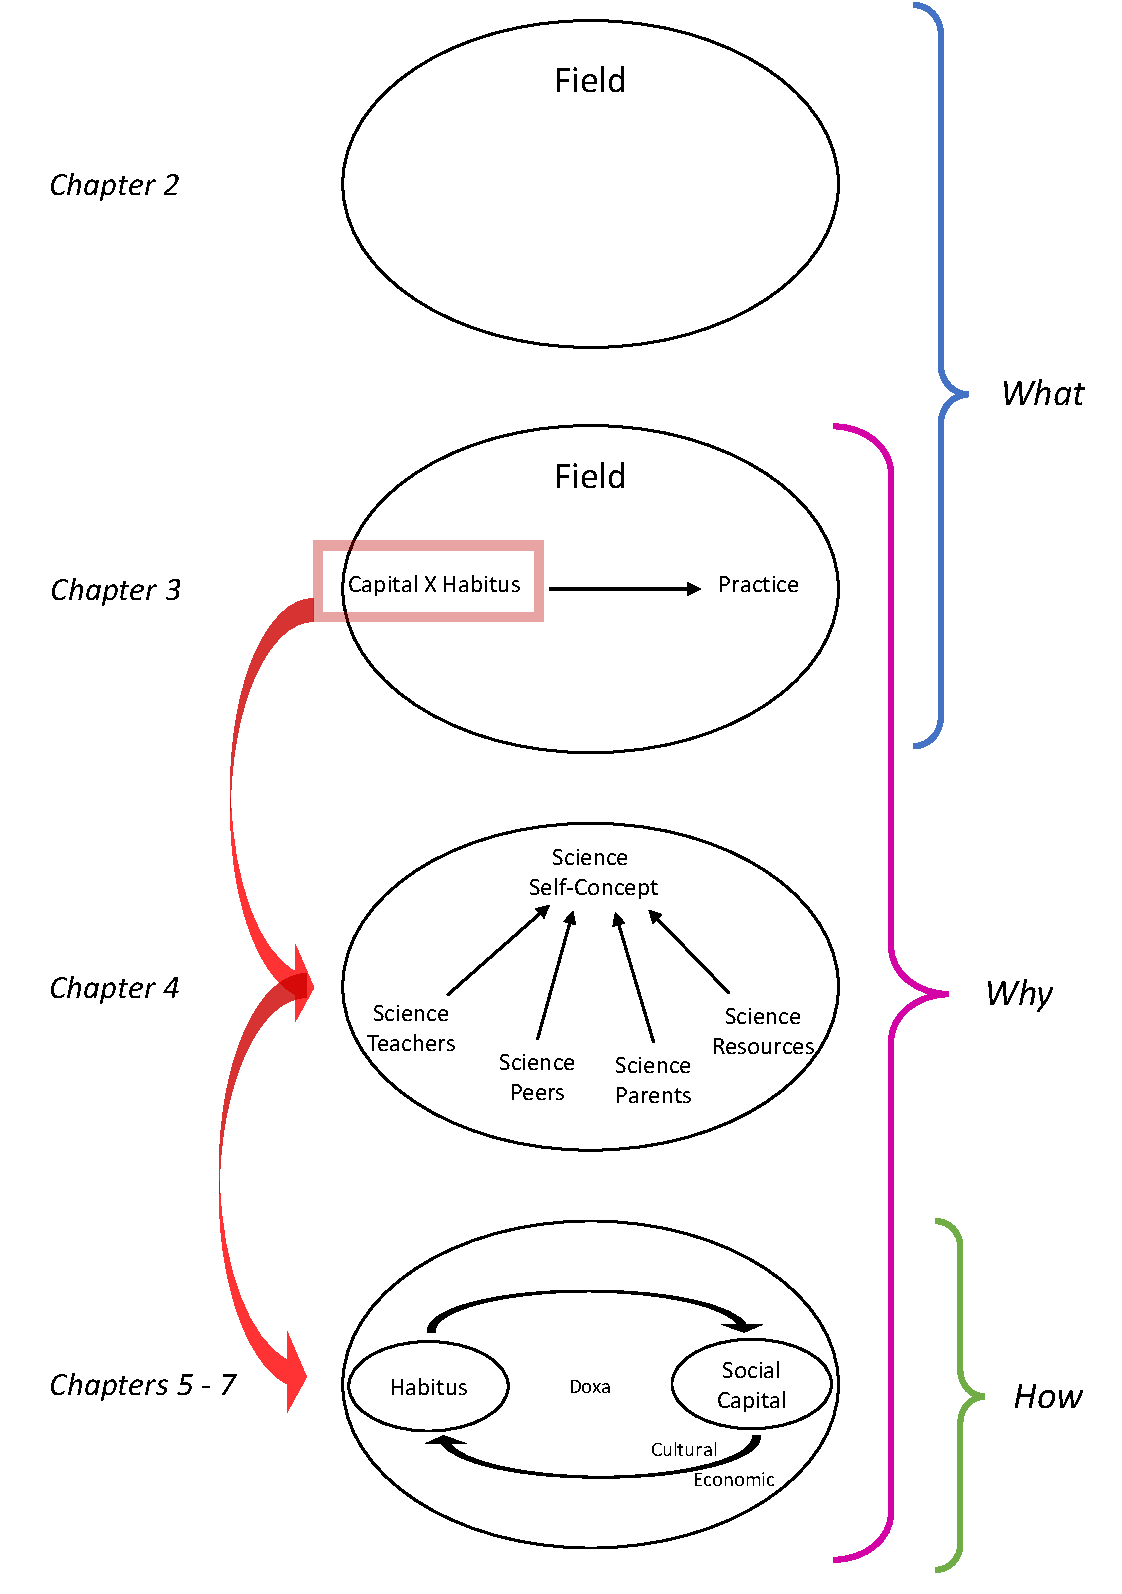
\includegraphics[width = \textwidth]{C1 - Introduction/Thesis_structure_guide.pdf}
    \caption{\textbf{Thesis Structure}. The guide to the structure of the thesis. The first conceptual model in is introduced in chapter 2, and focuses soley on understanding what the field of science participation looks like in New Zealand. Chapter 3 introduces a new conceptual model that incorporates the Bourdieusian concepts of capital and habitus in an attempt to explain what participation looks like, and potential reasons why it looks that way. Chapter 4 seeks to test one aspect of why participation differs according to Bourdieu's theory: the impact of science-related capital on student's belief that science is somewhere that they can be successful. In chapter 5 I build a new conceptual model that emphasises the importance of social capital and the reciprocal relationship shared with habitus, summarising its relevance for university science students in chapter 6. In chapter 7, I target each stage of this final conceptual model to offer potential opportunities to help provide equitable outcomes for students in science education. 
    }
    
    \label{fig:thesis_guide}
\end{figure}


The thesis itself is a combination of articles that have been submitting to journals and chapters written specifically for the thesis. As a result, some content may be repeated. Given the thesis was written over the period of three years, it is also possible that my understanding of Bourdieu's theory will be more developed in chapters written recently compared to older chapters. Each chapter will include a preamble which will place the following chapter in the context of which is was originally written, and in the context of the overall goals of the thesis. The following section provides an overview of how each one of my chapters fits within the goals of the thesis. 

Firstly, I seek to understand \textit{what} science participation looks like in New Zealand. Chapters 2 and 3 discuss the analysis of two big administrative data sets. The first data set was obtained through the Integrated Data Infrastructure (IDI) and represents all students from 2010 to 2016 studying Level 3 STEM standards in New Zealand high schools, while the second data set represents students studying who studied physics at undergraduate level from 2010 to 2016. In both of these chapters I employ network analysis as a method of untangling trends in complex data. For the purposes of this thesis, it was my intention for someone unfamiliar with network analysis to be able to understand the procedures behind the analysis, and more importantly, why it was used. 

Whilst both Chapters 2 and 3 detail \textit{what} science participation looks like in New Zealand, Chapter 3 also begins to delve into possible reasons for \textit{why} we see disparities in science participation. In Bourdieusian terms, Chapters 2 and 3 explain the state of the field of science education. Chapter 3 introduces Bourdieu's other concepts of capital and habitus as concepts that may explain \textit{why} the field is structured as it is, and the following chapters build on this model. Chapter 4 details the results of a survey that explored the relationships between forms of science-related capital and students' self-concept of science --- which I argue is the aspect of habitus that can be scrutinised through introspection. Chapter 5 details the development of a new conceptual model. This new model expands on the original Bourdieusian model outlined in Chapter 3, with the aim of highlighting the importance of social capital in particular, and the reciprocal relationship shared between capital and habitus. 

Following the development of the new conceptual model of capital and habitus in Chapter 5, Chapter 6 seeks to put the lived experiences of science students to the model. These students, purposefully sampled from the results of the survey discussed in Chapter 4, detail a range of different experiences. Through analysis of this qualitative data I try to unpack how science participation may be influenced by social location. 

After providing answers to the \textit{what} (Chapters 2 and 3) and the \textit{why} (Chapters 3 to 6), the final goal of the thesis is to suggest a \textit{how}: how can we improve the field of science education so that it is more equitable. Chapter 7 draws upon the conceptual model outlined in Chapter 5, the qualitative data detailed in Chapter 6, and the findings of previous research, to suggest opportunities for intervention that may make the field of science education more equitable. 


